\documentclass[11pt,a4paper]{article}
\usepackage[top=3cm, bottom=2cm, left=3cm, right=2cm]{geometry}
\usepackage[utf8]{inputenc}
% \usepackage[T1]{fontenc}
\usepackage{amsmath, amsfonts, amssymb}
\usepackage{siunitx}
\usepackage[brazil]{babel}
\usepackage{graphicx}
\usepackage[margin=10pt,font={small, it},labelfont=bf, textfont=it]{caption}
\usepackage[dvipsnames, svgnames]{xcolor}
\DeclareCaptionFont{MediumOrchid}{\color[svgnames]{MediumOrchid}}
\usepackage[pdftex]{hyperref}
\usepackage{natbib}
\bibliographystyle{plainnat}
\bibpunct{[}{]}{,}{s}{}{}
\usepackage{color}
\usepackage{footnote}
\usepackage{setspace}
\usepackage{booktabs}
\usepackage{multirow}
\usepackage{subfigure}
\usepackage{fancyhdr}
\usepackage{leading}
\usepackage{indentfirst}
\usepackage{wrapfig}
\usepackage{mdframed}
\usepackage{etoolbox}
\usepackage[version=4]{mhchem}
\usepackage{enumitem}
\usepackage{caption}
\usepackage{titlesec}




\titleformat{\section}{\LARGE\color{CarnationPink}}{\thesection}{1em}{}
\titleformat{\subsection}{\LARGE\color{CarnationPink}}{\thesubsection}{1em}{}


\DeclareCaptionLabelFormat{figuras}{\textcolor{CarnationPink}{Figura \arabic{figure}}}
\captionsetup[figure]{labelformat=figuras}

\makeatletter
\renewcommand\tagform@[1]{\maketag@@@{\color{CarnationPink}(#1)}}
\makeatother

\renewcommand{\theequation}{Eq. \arabic{equation}}
\renewcommand{\thefigure}{Fig. \arabic{figure}}
\renewcommand{\thesection}{\textcolor{CarnationPink}{\arabic{section}}}

\setlist[itemize]{label=\textcolor{CarnationPink}{$\mathbf{\square}$}}

\setlist[enumerate]{label=\textcolor{CarnationPink}{\arabic*.}, align=left}


\newcounter{exemplo}

\NewDocumentEnvironment{exemplo}{ O{} }{%
\allowbreak
\setlength{\parindent}{0pt}
  \begin{mdframed}[
  leftline=true,
  topline=false,
  rightline=false,
  bottomline=false,
  linewidth=2pt,
  linecolor=CarnationPink,
  frametitlerule=false,
  frametitlefont=\Large\bfseries\color{CarnationPink},
  frametitle={\color{CarnationPink}\normalfont\bfseries #1},
  ]
}{%
  \end{mdframed}
}

\setlength{\fboxsep}{5pt}
\setlength{\fboxrule}{1.5pt}
\usepackage{float}
\renewcommand{\thefootnote}{\alph{footnote}}
\usepackage{url}
\hypersetup{
	colorlinks=true,
	linkcolor=DarkTurquoise,
	filecolor=DarkTurquoise,      
	urlcolor=DarkTurquoise,
	citecolor=DarkTurquoise,
	pdftitle={Radioterapia}
}
\pagestyle{fancy}
\fancyhf{}
\renewcommand{\headrulewidth}{0pt}
\rfoot{Página \thepage}

\title{Física}
\author{Notas Rápidas \nocite{*}}
\date{\textit{Dalila Mendonça}}
\begin{document}
	\maketitle


\begin{exemplo}[Física]

    \begin{itemize}
        \item Isótopos estáveis possuem a razão nêutrons:protons de $1:1$ para $z <  20$ e 1.5:1 para núcleos mais pesados;
        
        \item O output de um tubo de raiox-x aumenta com o quadrado da voltagem do tubo  e linearmente com a corrente do tubo;
        
        \item A filtração inerente é especificada em termos de mm de Al e é normalmente de 0.5 mm de Al até 1.0 mm de Al;
        
        \item O feixe de elétrons que sai da cavidade de aceleração normalmente tem uma dispersão de energia de 1\% a 2\%. O bending magnet de \ang{270} permite o foco adequado de elétrons de energias ligeiramente diferentes e, portanto, menor ponto focal no alvo. Há também menos perda de intensidade do feixe de elétrons com o bending magnet de \ang{270}, embora com maior complexidade e custo de construção do linac. Ao usar apenas um bending magnet de \ang{90}, os elétrons de baixa energia seriam curvados ligeiramente mais do que os elétrons de alta energia, resultando assim em um grande ponto focal no alvo de raios-x. Um ponto focal maior, por sua vez, resultaria em uma ligeira degradação da nitidez da penumbra do feixe, o que é indesejável.
        
        \item As primeiras unidades combinadas de tratamento com RM usavam \ce{^{60}Co} porque expor o feixe de elétrons a um campo magnético externo é um problema de engenharia difícil, porém atualmente são utilizados AL's. Mesmo dentro do paciente, a presença do campo magnético afeta a distribuição da dose entregue devido às interações dos elétrons secundários com o campo magnético. Os implantes de metal podem estar sujeitos a aquecimento, bem como a forças magnéticas, e muitos implantes não são seguros para uso em nenhuma unidade de RM. Há uma limitação na movimentação de mesa quando comparados a Al's convencionais;
        
        \item De acordo com a AAPM TG-50, os MLC's são geralmente feitos de uma liga de tungstênio porque é dura, usinável, barata e tem uma das maiores densidades;
        
        \item A unidade de Hounsfield é dada por:
        
            \begin{equation*}
                HU = \left[\frac{\mu - \mu_{agua}}{\mu_{agua}}\right] \times 1000
            \end{equation*}
        \item Feixes de elétrons são mais prováveis de interagir com os elétrons orbitais das camadas mais externas do átomo. Quando uma partícula carregada interage com um átomo, a influência do campo de força coulombiano da partícula afeta o átomo como um todo. A maioria das interações são colisões “suaves” com elétrons da camada externa, transferindo apenas frações mínimas da energia cinética da partícula incidente. Esse processo costuma ser chamado de “aproximação de desaceleração contínua”.
        
        \item O controle automático de brilho em um modo de fluoroscopia do sistema de imagem kV montado em um gantry pode modificar kV e mAs. O objetivo do controle automático de brilho é obter a melhor qualidade possível da imagem de fluoroscopia alterando kV e mAs.
        
        \item O número de nêutrons produzidos por MU aumenta rapidamente com a energia do feixe, mas o espectro de energia dos nêutrons não tem uma forte dependência da energia do feixe, embora a energia média do nêutron aumente ligeiramente.
        
        \item A transmissão de um MLC é de 1 - 2\%; 
        
        \item O sistema de direcionamento do feixe compara as leituras das duas câmaras monitoras e as equaliza desviando o feixe garantindo a simetria do feixe. Ao fazê-lo, também mantém a taxa de dose, qualidade e saída, mas estes são simplesmente resultados de manter a simetria do feixe.
        
        \item MLCs com extremidades das lâminas arredondadas são projetadas para manter uma penumbra geométrica relativamente constante em diferentes posições da lâmina no feixe.
        
        \item A magnetron gera RF, enquanto A klystron requeruma fonte de RF (driver de RF), que ela amplificam. Um thyratron é um switch.
        
            \begin{itemize}
                \item Uma klystron amplifica as microondas de baixa potência em microondas de alta potência. À medida que os elétrons são enviados através de um tubo de drift, sua velocidade é modulada pelo campo elétrico alternado na frequência das micro-ondas de baixa potência entrantes, criando “montes” de elétrons. Os montes induzem cargas na cavidade final, criando microondas de maior potência na mesma frequência.
                
                \item A magnetron é um gerador de micro-ondas. Tem uma estrutura circular com um cátodo no centro e um ânodo na superfície externa composta por cavidades ressonantes. Os elétrons são produzidos no cátodo e são submetidos a um campo elétrico entre o ânodo e o cátodo. Um campo magnético estático é aplicado perpendicularmente ao campo elétrico e ao movimento dos elétrons. Os elétrons se movem em espirais em direção às cavidades, criando energia de micro-ondas, que é então enviada para o guia de onda acelerador.
            \end{itemize}
        
        \item A fotodesintegração é um processo nuclear no qual um núcleo atômico absorve um raio gama de alta energia, entra em um estado excitado e decai imediatamente emitindo uma partícula subatômica. Os nêutrons são produzidos nas reações ($\gamma$,n) por feixes de raios X de alta energia incidentes nos vários materiais do alvo, filtro de achatamento e colimadores. A contaminação por nêutrons aumenta rapidamente à medida que a energia do feixe aumenta de 10 para 20 MV e então permanece aproximadamente constante acima disso.
        
        \item A produção fluorescente $w$ é definida como a probabilidade de um átomo produzir radiação característica em vez de um elétron Auger: Alto Z, Alto $w$, portanto a emissão de raios-x característicos é mais provável; Baixo Z, baixo $w$ e portanto a emissão de elétrons auger é mais provável. 
        
        \item O \ce{SF6} é um dielétrico e evita arcos dentro do guia de ondas de transmissão que guia as micro-ondas de sua fonte para o guia de ondas de aceleração.
        
        \item Um linac usa microondas a 3.000 MHz ou 3 GHZ. Estes são chamados de microondas de banda S. Alguns aceleradores mais compactos, como o CyberKnife, usam micro-ondas da banda X em torno de 10 GHz. O tamanho do guia de ondas depende do comprimento de onda do micro-ondas, portanto, uma frequência mais alta implica em um guia de ondas mais curto.
        
        \item O efeito Cerenkov ocorre quando uma partícula carregada viaja em um meio a uma velocidade maior que a velocidade da luz nesse meio (nenhuma partícula massiva pode viajar mais rápido que a luz no vácuo). Nessa condição, a partícula carregada cria uma “onda de choque” eletromagnética, semelhante à onda de choque acústica quando um avião viaja mais rápido que a velocidade do som. A onda de choque eletromagnético aparece como uma explosão de radiação visível, conhecida como radiação de Cerenkov. Potencialmente, isso poderia ser usado para medir a posição e a intensidade da dose depositada.
        
        \item o \ce{^{192}Ir} decai emitindo uma partícula beta menos 95.1\% do tempo, emitindo na sequência radiação gama com energia média de 380 KeV. Nos restante do tempo (4.9\%) decai por captura eletrônica.
        
        \item Partículas carregadas viajando em um campo magnético experimentam a força de Lorentz, que atuará para curvar o caminho dos elétrons no plano perpendicular ao campo magnético. Não há efeito na velocidade do elétron. À medida que os linacs combinados com RM são introduzidos na clínica, os efeitos da força de Lorentz nos elétrons emitidos ao espalhamento Compton precisam ser considerados para calcular a distribuição de dose correta.
        
        \item A força nuclear forte entre nêutrons e prótons, nêutrons e nêutrons, prótons e prótons supera a força coulomb repulsiva entre prótons. 
        
        \item Na captura eletrônica, um elétron orbital é absorvido pelo núcleo, então a massa atômica permanece a mesma, mas o número atômico diminui em 1. O decaimento alfa mudaria tanto a massa atômica quanto o número atômico, o decaimento beta aumentaria o número atômico em 1 , e a emissão gama apenas converte um átomo do estado excitado.
        
        \item A diferença entre a massa de um núcleo e a soma das massas dos núcleons individuais livres que constituem esse núcleo é chamada de defeito de massa.
        
        \item Um cátodo aquecido e um alvo de metal estão presentes tanto nos aceleradores lineares quanto nos tubos de raios-X. Os ímãs de foco e as câmaras monitoras são encontrados apenas nos linacs. Apenas os tubos de raios X possuem ânodos rotativos e tubos de vidro.
        
        \item A forma de um filtro bowtie em uma tomografia permite atenuar seletivamente os fótons em função do ângulo do raio-x emitido pela fonte. Todos os filtros irão absorver raios-x de baixa energia. A forma do filtro geralmente é mais espessa onde os raios X incidiriam sobre a periferia do paciente, reduzindo assim o fluxo e, portanto, a dose nas periferias do paciente.
        
        \item A saída de um tubo de raio    s X aumenta linearmente com a corrente do tubo e aumenta com o quadrado da voltagem do tubo.
        
        \item Um ânodo rotativo é usado para espalhar o aquecimento sobre uma grande área do ânodo. Da mesma forma, um ânodo angular é usado para que uma área maior do ânodo possa ser usada, mantendo o ponto focal aparente suficientemente pequeno. O corpo do ânodo é feito de materiais com alta capacidade de armazenamento de calor, como molibdênio ou grafite.
        
        \item Em um linac, o output pode mudar significativamente após a substituição de uma câmara de íons devido a diferenças na quantidade de gás entre as antigas e as novas câmaras. Portanto, a saída da máquina precisará ser ajustada/recalibrada após a substituição da câmara. A simetria e planura são uma função do direcionamento do feixe, e a energia do feixe é determinada pelo potencial de aceleração e pelo alvo.
        
        \item Quanto ao alvo em um linac, um número atômico alto aumentará a frequência de produção de raios-x devido ao aumento da seção transversal de bremsstrahlung. Diferentes espessuras de alvo são usadas para cada energia de fóton desejada devido ao fato de que a energia dos elétrons incidentes será diferente.
        
        \item Os elétrons da gun de elétrons são acelerados através das guia de ondas, transportados através de ímãs de flexão e incidem sobre o alvo. Os fótons provenientes das interações no alvo saem pela janela de saída e são colimados pelos colimadores primários, atravessam o filtro aplanador e a câmara de ionização e são colimados pelos jaws superior e inferior.
        
        \item Uma mesa de tratamento padrão possui quatro graus de liberdade que permite translações laterais, verticais e longitudinais e rotações em torno do eixo vertical. Uma mesa de tratamento com seis graus de liberdade também permite rotações em torno do eixo lateral e longitudinal (inclinação), o que facilita o alinhamento do paciente em tratamentos SBRT e SRS guiados por imagem.
        
        \item O modulador inclui a rede de formação de pulso e um tubo de switch conhecido como tyratron de hidrogênio. Pulsos de alta potência e curta duração da seção do modulador são entregues à klystron e simultaneamente à gun de elétrons.
        
        \item Existem três áreas de transmissão de MLC: através da extremidade arredondada da lâmina, através do centro da lâmina (vazamento intralâmina) e entre lâminas adjacentes (vazamento interlâminas). No modelo tongue and groove, a “tongue” (língua) de uma lâmina se entrelaça com a “groove” (ranhura) de uma lâmina adjacente na mesma margem, na tentativa de manter o vazamento interlâminas aceitavelmente baixo, da ordem de 3 a 4\%.
        
        \item À medida que a energia do feixe de raios X aumenta, a distribuição de fluência será mais direcionada para frente e então feixes de energia mais alta precisam de filtros aplanadores mais espessos. Portanto, se um filtro aplanador de 6 MV for usado para o feixe de 15 MV, a magnitude dos ``chifres'' diminuirá devido à atenuação insuficiente ao longo do CAX em relação aos pontos fora do eixo, e a taxa de dose aumentará devido a uma diminuição da espessura do filtro.
        
        \item Para terapia de feixe de elétrons, todos os elétrons do tubo acelerador são usados para terapia. Para a terapia de fótons, no entanto, os elétrons devem ser convertidos em fótons no alvo por meio de interações de bremsstrahlung, e apenas uma fração da energia do elétron é convertida. Portanto, correntes de acelerador muito mais altas são necessárias para terapia de fótons do que para terapia de elétrons. A eficiência da produção de raios-x bremsstrahlung aumenta tanto com o número atômico do alvo quanto com a energia do feixe de elétrons. Portanto, um feixe de fótons de 15 MV requer uma corrente de elétrons menor do que um feixe de 6 MV. A eficiência de conversão para a produção de bremsstrahlung é de aproximadamente 1\% a 100 kVp e 70\% a 20 MeV.
        
        \item As lâminas mais estreitas são mais vantajosas em tratamentos de pequenas lesões em pequenas profundidades pois para tumores pequenos e irregulares, a modelagem de campo mais precisa é claramente mais importante do que para tumores maiores, mas em profundidades maiores, a dispersão do feixe anula em grande parte a definição de campo mais nítido alcançadas por lâminas do MLC pequenas.
        
        \item A probabilidade de uma interação fotoelétrica é proporcional ao cubo do número atômico do material (Z) dividido pela energia do fóton (E), ou (Z/E)\textsuperscript{3}. O osso tem o maior número atômico efetivo comparado ao músculo, a gordura e a água e, portanto, o maior coeficiente de interação, resultando na maior dose absorvida para a mesma fluência de fótons de 100 kV.
        
        \item De acordo com a equação do poder de freamento de mássico de Bethe, a deposição de energia para partículas carregadas aumenta com o quadrado da carga e inversamente com a velocidade, quando a energia da partícula diminui. O aumento maciço no poder de freamento dos íons de carbono dá a ele uma queda de pico de Bragg muito mais acentuada do que para prótons, pósitrons, elétrons e partículas alfa.
        
        \item O espalhamento Compton é dominante na água para energias de fótons entre 25 keV a 25 MeV e depende da densidade eletrônica. O efeito fotoelétrico é dominante abaixo de 25 keV e é proporcional a Z\textsuperscript{3} e 1/E\textsuperscript{3}.
        
        \item O coeficiente de atenuação mássico é maior para fótons de baixa energia e meios com alto número atômico devido à predominância de interações fotoelétricas nessas condições. Um MeV está na faixa de Compton, portanto o ($\mu/\rho$) de chumbo e água não difere muito, já que a interação Compton é independente do número atômico. Em 10 MeV, ocorre o domínio da produção de pares, especialmente para meios com alto número atômico.
        
        \item A exposição refere-se especificamente à ionização no ar causada por fótons menores que 3 MeV.
        
        \item Ciclotrons médicos são usados para produzir radioisótopos tipicamente de vida curta que são ricos em prótons. F-18 pode ser produzido em um ciclotron bombardeando O-18 com prótons. O Rn-222 faz parte da série natural de decaimento do urânio. Tc-99m é o produto de decaimento do molibdênio-99, que é produzido em reações nucleares. Co-60 e Ir-192 também são produzidos em reator, criados a partir do bombardeio de Co-59 e Ir-191, respectivamente, com nêutrons.
        
        \item Ciclotrons bombardeiam núcleos estáveis com prótons, colocando o radioisótopo resultante abaixo da linha de estabilidade. Portanto, o mecanismo de decaimento típico é via emissão de pósitrons. Muitos dos radioisótopos de vida curta usados em imagens de PET são produzidos por ciclotrons.
        
        \item O joule é a unidade SI para energia, trabalho e calor. O gray é a unidade SI para dose de radiação e 1 Gy = 1 J/kg = 1 kg m\textsuperscript{2}/s\textsuperscript{2}.
        
        \item No decaimento $\mathrm{\beta}^-$, um nêutron decai em um próton, um elétron e um antineutrino e, possivelmente, raios gama. Com o próton adicional, o número atômico aumenta em 1, mas a soma de prótons e nêutrons, A, permanece inalterada.
        
        \item A energia de um fóton é inversamente proporcional ao comprimento de onda da onda eletromagnética que representa esse fóton. E = h x frequência = h (c / $\lambda$).
        
        \item Os isótopos são estáveis, ou seja, improváveis de decair, se tiverem uma proporção de nêutrons:prótons de 1:1 para isótopos de baixa massa atômica e 1,5:1 para elementos pesados. Isso é chamado de linha ou faixa de estabilidade. Acima da linha, onde há mais nêutrons do que prótons, o decaimento beta menos é mais provável, e abaixo da linha, onde há mais prótons do que nêutrons, é provável o decaimento beta mais (pósitrons).
        
        \item A emissão de $K_\alpha$ requer que um elétron na camada K seja arrancado por elétrons incidentes com uma energia mínima igual a energia de ligação da camada K.
        
        \item Raios-x característicos são produzidos quando uma vacância da camada interna do elétron é preenchida por um elétron da camada externa. No entanto, às vezes a energia não é liberada como um raio-x, mas transferida para um elétron que é ejetado do átomo. Esses elétrons são chamados de elétrons Auger.
        
        \item Existem dois tipos de filtração em um tubo de raios X. A primeira é a filtração inerente, que vem da janela, envolucro e óleo presentes no próprio tubo de raios-x. A filtração inerente é geralmente de cerca de 0,5 a 1,0 mm de equivalente de alumínio. A segunda é a filtração adicional, que consiste em folhas de metal adicionadas ao feixe para remover os raios X de baixa energia.
        
        \item O ânodo de um tubo de raios X é onde os raios X são produzidos. Como os raios X são produzidos por meio de interações de bremsstrahlung, um número atômico alto é desejável. Um alto ponto de fusão é necessário, pois a grande maioria da energia dos elétrons que atingem o ânodo é convertida em calor. 
        
        \item O feixe de elétrons que sai guia aceleradora normalmente tem uma distribuição de energia de 1\% a 2\%. O ímã de flexão de \ang{270} permite o foco adequado de elétrons de energias ligeiramente diferentes e, portanto, um  ponto focal menor no alvo. Há também menos perda de intensidade do feixe de elétrons com o ímã de flexão de \ang{270}, embora tenha uma maior complexidade e custo na construção do linac. Ao usar apenas um ímã de flexão de \ang{90}, os elétrons de baixa energia seriam dobrados ligeiramente mais do que os elétrons de alta energia, resultando assim em um grande tamanho do ponto focal no alvo de raios-x. Um ponto focal maior, por sua vez, resultaria em uma ligeira degradação da nitidez da penumbra do feixe, o que é indesejável.
        
        \item O feixe de raios X ou o feixe de elétrons incide nas câmaras monitoras de dose. O sistema de monitoramento consiste em várias câmaras de ionização ou uma única câmara com várias placas. Embora as câmaras sejam geralmente do tipo transmissão, ou seja, câmaras planas de placas paralelas para cobrir todo o feixe, câmaras cilíndricas dedais também têm sido usadas em alguns linacs. A função da câmara de íons é monitorar a taxa de dose, a dose integrada e a simetria do campo.
        
        \item Considerando dois linacs, o Linac A tem um MLC que também serve como um colimador secundário. O Linac B tem uma jaws como colimador secundário e um MLC terciário para moldar ainda mais o feixe. Em um determinado SSD, haveria mais espaço entre o cabeçote do gantry e o paciente para o linac A. Como haverá jaws e MLCs no linac B, haverá menos espaço entre a cabeça do gantry e o paciente em um determinado SSD. No entanto, não há nenhuma razão de engenharia para que o linac A tenha lâminas que viajam mais rápido ou posições de lâminas que possam ser definidas com mais precisão. Da mesma forma, não há nenhuma razão de engenharia para que apenas o MLC no linac A seja capaz de se mover dinamicamente durante o feixe, como ocorre para o sliding window IMRT e VMAT. 
        
        \item Comparando um linac com e sem filtro aplanador, o linac sem um filtro aplanador para atenuar o feixe, terá uma taxa de dose será maior e a energia do feixe será menor. Como o objetivo de um filtro aplanador é tornar a intensidade do fóton “plana” em uma determinada profundidade, a falta de um filtro aplanador resultará em intensidades de fótons mais altas no eixo central do feixe.
        
        \item As primeiras unidades de tratamento combinadas com RM usavam \ce{^{60}Co} porque expor o feixe de elétrons a um campo magnético externo é um problema de engenharia difícil. Mesmo dentro do paciente, a presença do campo magnético afeta a distribuição da dose entregue devido às interações dos elétrons secundários com o campo magnético. Os implantes de metal podem estar sujeitos a aquecimento, bem como a forças magnéticas, e muitos implantes não são seguros para uso em nenhuma unidade de RM.
        
        \item A produção de Bremsstrahlung é proporcional a EZ\textsuperscript{2}, onde E é a energia do elétron incidente e Z é o número atômico do alvo.
        
        \item O efeito anódico ocorre devido à auto-atenuação não uniforme dentro do ânodo angulado usado na geração do feixe de kV. Os feixes MV, pelo contrário, utilizam um alvo uniforme de transmissão e não experimentam o efeito anódico.
        
        \item De acordo com a AAPM TG-50, os colimadores multi-lâminas (MLC) são geralmente feitos de uma liga de tungstênio porque é dura, usinável, barata e tem uma das maiores densidades que qualquer outro material.
        
        \item À medida que um feixe de fótons polienergéticos atravessa um material homogêneo, os fótons de menor energia são preferencialmente atenuados, de modo que a energia média do feixe aumenta. Portanto, o primeiro HVL será o menor e o HVL aumentará com o aumento da espessura do material.
        
        \item Quando uma partícula carregada interage com um átomo, a influência do campo de força coulombiano da partícula afeta o átomo como um todo. A maioria das interações são colisões “suaves” com elétrons da camada externa, transferindo apenas frações mínimas da energia cinética da partícula incidente. Esse processo costuma ser chamado de “aproximação de desaceleração contínua” ``continuous slowing-down approximation''.
        
        \item O ouro tem um número atômico alto e é um material de alta densidade, portanto as interações fotoelétricas são significativas, resultando em alto contraste em uma tomografia computadorizada ou em uma imagem planar kV entre o marcador fiducial feito com ouro e o tecido no qual está implantado.
        
        \item Em uma interação de espalhamento Compton, um fóton incidente interage com um elétron livre. Parte da energia do fóton é transferida para o elétron e o restante da energia permanece com o fóton espalhado. Devido à conservação de energia e momento, o elétron pode ser desviado entre +90 e –90 graus. O fóton pode ser desviado por qualquer ângulo. Um ângulo de espalhamento de 180 graus é aquele em que a energia máxima foi transferida pelo fóton para o elétron.
        
        \item A produção de pares ocorre quando um fóton com energia acima de um limiar de 1,022 MeV interage com o campo coulombiano ao redor de um núcleo. O fóton desaparece e um par elétron-pósitron é produzido.
        
        \item À medida que a energia do fóton MV aumenta, a profundidade de d\textsubscript{max} aumenta e a dose de superfície diminui, devido ao aumento da energia média dos elétrons secundários liberados pelas interações dos fótons com o material

    \end{itemize}

\end{exemplo}

\begin{exemplo}[Dosimetria]
    \begin{itemize}
        \item O filme radiocrômico tem muitas vantagens que o tornam amplamente utilizado para aplicações dosimétricas. O fato de ser auto-revelável e insensível à luz ambiente torna-o mais fácil de manusear do que o filme radiográfico. Sua alta resolução espacial, equivalência de tecido e falta de dependência de energia o torna bom para uma ampla gama de medições dosimétricas.
        
        \item A densidade do ar na cavidade da câmara de ionização depende da temperatura e da pressão, de acordo com a lei dos gases. A densidade ou massa de ar no volume da câmara aumentará à medida que a temperatura diminuir ou a pressão aumentar. A exposição é definida como a carga de ionização coletada por unidade de massa de ar. Portanto, a leitura da câmara para uma determinada exposição aumentará à medida que a temperatura diminuir ou a pressão aumentar.
        
        \item A câmara de ionização mede de fato a ionização causada pelo feixe de radiação, que não coincide exatamente com a dose de radiação. A razão do poder de freamento, que depende da energia e muda com a profundidade, pode ser usada para converter a ionização de profundidade percentual (PDI) em dose de profundidade percentual (PDD).
        
        \item Quando um chip OSLD é irradiado, um elétron da banda de valência pode obter energia suficiente para se mover para a banda de condução. À medida que cai da banda de condução, pode ficar preso por uma armadilha de elétrons. Essas armadilhas são causadas por imperfeições na estrutura de rede do material. A luz visível de um determinado comprimento de onda é usada ao ler um chip OSLD, que libera o elétron preso. A diferença de energia entre o estado preso e a banda de valência é emitida como luz visível.
        
        \item Os dosímetros absolutos podem determinar a dose de radiação sem referência a outro dosímetro. Uma câmara de ionização de ar livre é freqüentemente usada por laboratórios de padrões e mede a carga elétrica resultante da ionização do ar em um campo de radiação. Os calorímetros medem o calor resultante da deposição de energia de radiação. Um dosímetro Fricke é um dosímetro químico, onde a oxidação de íons ferrosos em íons férricos em um campo de radiação é medida.
        
        \item A penumbra física é especificada pela largura lateral dos níveis de isodose (90\% a 20\%) perto das bordas do campo. É influenciado pela penumbra geométrica (que varia com a dimensão da fonte, profundidade e SDD), energia do feixe e equilíbrio eletrônico lateral.
        
        \item A fluência é definida como o número de partículas incidentes em uma esfera de área de seção transversal dA e possui unidades 1/m. A fluência de energia é a energia radiante incidente em uma esfera de área de seção transversal dA com unidades de J/m\textsuperscript{2}. A taxa de fluência de energia tem unidades J/m\textsuperscript{2}s.
        
        \item O equilíbrio das partículas carregadas pode ser perdido se as partículas secundárias criadas a partir das interações dos fótons dentro do material puderem se espalhar para longe das bordas do campo. Energias de fótons mais altas resultam em energias médias mais altas de elétrons secundários, permitindo que viajem mais longe. Da mesma forma, se o tamanho do campo for pequeno em relação à distância média que os elétrons secundários podem percorrer, o equilíbrio das partículas carregadas pode ser perdido.
        
        \item kQ auxilia na conversão do termo ND,w da energia do feixe Co-60 utilizado na calibração para a qualidade do feixe da máquina do usuário (Q) que está sendo calibrada.
        
        \item A medida que o volume de uma câmara de ionização aumenta a quantidade de carga no volume gerado irá aumentar, pois uma câmara de maior volume gerará mais carga para a mesma dose dada, pois há um maior volume de gás sendo irradiado.
        
        \item Para dosimetria in-vivo no monitoramento da dose recebida em um marcapasso uma opção a ser utilizada, além dos diodos são os dosímetros luminescentes oticamente estimulados OSLD. Os dosímetros luminescentes estimulados opticamente são pequenos, não requerem voltagem aplicada, têm uma dose-resposta linear e podem ser lidos em cerca de 30 minutos após a irradiação. As câmaras de ionização, como as câmaras Farmer ou de placas paralelas, usam alta voltagem, portanto são perigosas, além de volumosas e difíceis de usar. O filme radiocrômico requer alta dose em comparação com a dose recebida por um marca-passo cardíaco durante o tratamento de radioterapia.
        
        \item Dosímetros termoluminescentes (TLDs) e dosímetros luminescentes opticamente estimulados (OSLDs) são frequentemente usados para medições de dose de superfície in vivo. Câmaras de placas paralelas podem ser usadas para medições de dose de superfície em um fantoma, embora as câmaras de extrapolação sejam o padrão-ouro.
        
        \item De acordo com o adendo ao protocolo de calibração AAPM Task Group 51, a correção de recombinação iônica é maior para feixes de fótons sem filtro aplanador em comparação com feixes planos.
        
        \item Em uma leitura realizada com uma câmara de ionização, à medida que a pressão aumenta, a densidade do ar na câmara aumentará, resultando em um aumento correspondente na carga medida.
        
        \item KERMA é a energia cinética liberada na matéria e representa a energia transferida dos fótons incidentes para os elétrons que são acionados por uma interação fóton-elétron. Esses elétrons transferem grande parte de sua energia localmente, mas não de uma só vez. A energia é depositada ao longo do comprimento do caminho percorrido do elétron, então o KERMA, a energia inicialmente transferida, é maior na região onde os elétrons ainda não depositaram toda a sua dose (a região de acúmulo - build up).
        
        \item A fluência é o número (dN) de partículas incidentes em uma esfera de área de seção transversal (dA).
        
        \item Os dosímetros OSLDs fornecem um meio para medições de dose in vivo, mas não em tempo real. No entanto, a resposta desses dosímetros diminui após a irradiação. Para medir a dose com precisão e reprodutibilidade, as medidas com  OSLD devem ser feitas após o término desse período de enfraquecimento (na ordem de cerca de uma hora). OSLDs exibem uma resposta de dose linear, independência de energia para feixes de MV, bem como uma insensibilidade à taxa de dose e temperatura.
        
        \item Uma câmara de ionização de placas paralelas é o melhor instrumento para medições de output de elétrons. Seu tamanho de volume sensível deve ser muito menor que o tamanho do cutout. Uma câmara cilíndrica também pode ser usada para energias de elétrons mais altas, desde que o cutout seja muito maior em tamanho do que a área de coleta da câmara.
        
        \item Dosímetros luminescentes opticamente estimulados (OSLDs) ou dosímetros termoluminescentes (TLDs) são os meios mais comuns de medir a dose do marcapasso em um paciente. Um medidor de nêutrons é volumoso e só capturaria a dose de nêutrons. As câmaras ionização usam alta voltagem, o que é perigoso para o paciente. O filme radiocrômico é impreciso para pequenas doses.
        
        \item A leitura de carga totalmente corrigida de uma câmara de íons é fornecida em AAPM TG-51 como: M = P\textsubscript{ion} P\textsubscript{TP} P\textsubscript{elec} P\textsubscript{pol} M\textsubscript{raw}. M\textsubscript{raw} é a leitura bruta da câmara e P\textsubscript{ion} é o fator responsável pelo fato de que parte da ionização que ocorre na câmara resulta em recombinação antes de ser medida pela câmara. P\textsubscript{ion} é uma função da taxa de dose e da tensão de polarização e é medido pela aquisição de medições em duas configurações diferentes de tensão de polarização da câmara.
        
        \item Os diodos de silício são pequenos o suficiente para medir campos pequenos. A placa paralela e as câmaras farmer são muito grandes e resultariam em efeitos de média de volume, subestimando o sinal. Uma câmara de ionização de ar livre é usada para medir a exposição no ar, e uma câmara de poço é usada para calibração de fontes radioativas.
        
        \item Os tratamentos de TBI são frequentemente administrados em SSDs estendidos, de até 400 cm, e a dosimetria in vivo pode indicar se o paciente foi posicionado na distância correta da fonte. A dosimetria in vivo pode informar à equipe que o tratamento não estava sendo administrado conforme prescrito, mas não pode verificar se a dose prescrita está correta. Um único dosímetro no ponto de prescrição não pode fornecer informações sobre a homogeneidade da dose em todo o paciente. Nesse caso, os dosímetros precisariam ser colocados em vários locais ao longo do corpo.
        
    \end{itemize}
\end{exemplo}



\begin{exemplo}[Radioterapia]
    \begin{itemize}
        \item Para feixes de fótons MV, a profundidade da dose máxima aumenta com o aumento da energia.
        
        \item Uma aproximação geral para um feixe de raios X de 6 MV é que cada centímetro de tecido ausente resulta em 3,5\% menos atenuação;
        
        \item Em feixes de fótons onde existe um gap de ar entre o bolus e a superfície, o efeito do bolus é reduzido à medida que o gap de ar aumenta, resultando no aumento da profundidade da dose máxima e na diminuição da dose de superfície.
        
        \item A taxa de dose para um feixe FFF pode ser de três a cinco vezes maior quando comparados à feixes com filtro aplanador, o que resulta em tratamentos mais rápidos. A ausência de um filtro aplanador reduz significativamente a quantidade de radiação espalhada no cabeçote da máquina, o que pode reduzir a dose de corpo inteiro do paciente e também facilitar a modelagem do feixe em um sistema de planejamento de tratamento. A dose na superfície é ligeiramente aumentada para um feixe FFF, embora a diferença seja pequena e possa ser clinicamente insignificante.
        
        \item Uma camada de tecido pulmonar atenuará menos o feixe do que uma camada de tecido mole da mesma espessura. Portanto, o comprimento do caminho equivalente na água será menor para o pulmão do que para o tecido mole.
        
        \item A configuração do colimador informada pelo linac é o tamanho da projeção os jaws no isocentro da máquina. Em outras palavras, o tamanho da abertura física dos jows que seriam medidos com uma régua no cabeçote do Al seria muito menor do que a configuração relatada do colimador. A configuração do colimador é independente da posição do paciente, embora certamente o paciente possa ser colocado de forma que o isocentro esteja na entrada ou na superfície de saída.
        
        \item Pontos de cálculo colocados em regiões fora do campo, próximos a borda do campo, próximos a interfaces de heterogeneidade e na superfície do paciente são áreas típicas de fraqueza para algoritmos de cálculo de dose usados no cálculo de dose TPS e MU. As incertezas dos cálculos de dose nessas áreas são relativamente grandes porque o equilíbrio eletrônico não existe (por exemplo, pontos na superfície do paciente, perto da borda do campo e interface de heterogeneidade) ou a dose espalhada é o principal componente da dose (dose fora do campo). A precisão dos cálculos de dose em TPS para essas áreas deve ser verificada com medições.
        
        \item Ao converter de uma configuração de SAD de 100 cm para um setup de SSD a 100 cm, você está aumentando a SSD e a PDP aumenta à medida que o SSD aumenta, portanto, o ponto quente diminuirá. À medida que aumenta a espessura do paciente, mais dose será necessária para tratar na profundidade do meio do DAP, aumentando o ponto quente. Um feixe de alta energia é mais penetrante do que um feixe de baixa energia, portanto, para tratar na profundidade do meio do DAP, o ponto quente diminuirá à medida que a energia do feixe aumentar.
        
        \item Pacientes de próstata que possuem marca-passo devem ser tratados com feixes de fótons com energia de até 10 MV  porque nêutrons dispersos que penetram na blindagem do linac podem desencadear irregularidades no marcapasso. Observou-se que nêutrons dispersos podem desencadear irregularidades no marca-passo. Números significativos de nêutrons são produzidos apenas para feixes de fótons de energias acima de 10 MeV.
        
        \item Linacs modernos normalmente usam folhas de espalhamento dupla.
        
        \item As folhas usam uma combinação de materiais de alto Z e baixo Z para aumentar a dispersão, mas também minimizar a produção de bremsstrahlung.
        
        \item No modo de elétrons, o alvo e o filtro aplanador são girados para fora do caminho do feixe e a folha espalhadora é girada para dentro.
    
        \item Existem diversas folhas espalhadoras na cabeça da máquina para lidar com as diferentes energias de elétrons existentes no equipamento.
        
        \item Uma blindagem ocular de tungstênio pode ser utilizada para blindar os elétrons do feixe externo, mas não seria espessa o suficiente para blindar os raios gama Co-60 ou raios-x MV.
        
        \item A profundidade estimada para elétrons na PDP de 90\% é de cerca de E(MeV) / 3,2.
        
        \item Em relação à incidência normal, a incidência oblíqua em feixes de elétrons aumentará a dose de superfície, mas diminuirá a profundidade de Dmax e D90\% distal.
        
        \item Para tamanhos de campo de elétrons maiores do que o alcance prático do feixe de elétrons, a curva de PDP permanece relativamente constante com o aumento do tamanho do campo, uma vez que os elétrons da periferia do campo não são espalhados o suficiente para contribuir para a dose de profundidade do eixo central. Quando o campo é reduzido abaixo do necessário para manter equilíbrio de espalhamento lateral, a taxa de dose diminui, Dmax se aproxima da superfície e a curva PDP muda. Além disso, quando o tamanho do campo eletrônico (e-insert) é menor que o alcance prático do elétron, a saída pode ser sensível ao formato do campo.
        
        \item Tratamentos de TSI utilizam dois campos angulados pois a contaminação com os raios-x  bremsstrahlung são direcionados para a frente e são maiores ao longo do eixo central do feixe, portanto, a inclinação do gantry permite que esses raios-x sejam direcionados acima da cabeça do paciente e abaixo de seus pés. O uso de campos múltiplos também melhora a uniformidade na profundidade de prescrição.
        
        \item Para feixes de elétrons o retroespalhamento aumenta com o aumento do número atômico (Z). O bolus tem um número atômico efetivo semelhante ao da água (~8), seguido do alumínio (Z=13) e do chumbo (Z=82). Ao projetar blindagem interna para terapias com feixes de elétrons, as propriedades de retroespalhamento dos materiais são consideradas. Muitas vezes, materiais compostos, por exemplo, chumbo e bólus, são usados na blindagem para reduzir a espessura fa blindagem. Nesse caso, o material de Z mais alto deve estar no final do alcance do elétron, ou seja, adjacente ao OAR, pois retroespalhará no material de Z mais baixo.
        
        \item A AAPM TG-203 recomenda que a dose cumulativa para um dispositivo cardíaco implantado (CDI) seja menor ou igual a 500 cGy, ou o limite de dose recomendado pelo fabricante, caso seja maior.
        
        
        \item Em um tratamento de SBRT na base do pulmão, devido à proximidade do diafragma, é difícil saber a extensão do movimento do alvo sem uma imagem 4D. Embora possa ser útil para uma massa mediastinal, o erro de configuração tem menos efeito ao longo do tempo com o fracionamento convencional, e o tempo extra e a dose de uma CBCT 4D diária não são justificados. Para SRS craniano, o alvo é fixado dentro do crânio e um 4D não fornece informações extras. As maiores preocupações para o PBI (tratamento de mama parcial) são a dose no coração e no pulmão, mas uma margem adequada e a consideração do DIBH (inspiração profunda) são mais apropriadas do que 4D para garantir a cobertura adequada.
        
        \item De acordo com o relatório do AAPM Task Group 180 (Image Guidance Doses Delivered during Radiotherapy: Quantification, Management, and Reduction), a MV-CBCT pode resultar em uma dose maior que 10 cGy, dependendo do local da imagem e do protocolo.
        
        \item A imagem de superfície óptica (OSI) usa luz, não utiliza radiação ionizante. Portanto, pode ser utilizado para monitoramento contínuo durante o tratamento sem preocupação com danos ao paciente. Um caso de uso para monitoramento contínuo é o monitoramento do movimento respiratório para tratamentos de gating e inspiração profunda.
        
        \item É verdade que o OSI pode ser usado por RTTs dentro da sala, ao contrário da imagem baseada em raios-x, embora isso seja uma vantagem. OSI tem boa precisão para detecção de movimento. No entanto, o OSI usa a face como um substituto para a posição da lesão para SRS craniano, o que pode ser desvantajoso, pois você não está monitorando diretamente a própria lesão. O movimento da face, ou aspectos da face, não necessariamente se correlacionam diretamente com a posição da lesão.
        
        \item Monitoramento por infravermelho de marcadores, imagem de superfície óptica e métodos de espirometria que usam controle de respiração ativa são opções para realizar DIBH.
        
        \item Um algoritmo de sequenciamento de lâminas converte a fluência ideal calculada pelo algoritmo de otimização em um padrão de fluência que pode ser entregue pelo linac. Ele faz isso levando em consideração as características físicas do MLC a ser utilizado, como largura da lâmina, comprimento, número de lâminas disponíveis e restrições de velocidade da lâmina.
        \item Em gráficos de otimização o valor mínimo global da função objetivo do otimizador representa o melhor resultado da otimização caso o sistema de planejamento do tratamento fosse projetado para minimizar o valor da função objetivo.
        
        \item A entrega do tratamento com MLC no modo step and shoot é caracterizada pelo feixe sendo desligado conforme as lâminas do MLC se movem de um ponto de controle para o próximo. A entrega do MLC com sliding window envolve fazer com que as lâminas do MLC se movam enquanto o feixe permanece ligado de um ponto de controle para o próximo.
        
        \item Os gradientes de dose atingíveis para um plano IMRT de pórtico fixo ou um plano VMAT são da ordem de 10\% / mm. Se for necessário poupar mais um órgão crítico próximo, a cobertura do alvo pode precisar ser sacrificada.
        
        \item Quando um tratamento de TBI é movido de uma distância grande para uma menor, o PDP diminui à medida que a SSD diminui. A uniformidade da dose piora à medida que a PDP diminui utilizando campos paralelos opostos.
        
        \item Em um tratamento de TBI, ao usar feixes bilaterais com o paciente em decúbito dorsal, os braços podem atuar como um bloqueio para o pulmão. A uniformidade da dose será tipicamente pior, pois a faixa de espessuras variará mais na direção lateral do que na direção AP/PA; Daí o aumento da necessidade de compensação tecidual.
        
        \item O dicloreto de Ra-223 (XOFIGO) está disponível em forma de injeção utilizada para tratar a metástase óssea de câncer de próstata. Ra-223 é um emissor alfa e pode ser usado para tratar câncer ósseo. Ir-192, I-125 e Pd-103 são emissores gama normalmente usados como fontes seladas para braquiterapia. I-131 é um emissor gama e beta ingerido para o tratamento da tireoide.
        
        \item Quanto aos feixes utilizados em IORT (intraoperatória), Os elétrons geralmente têm energias na faixa de 4 a 12 MeV, o que resultará em maior penetração e homogeneidade de dose do que se pode obter de um afterloading HDR ou técnicas de fótons de quilovoltagem. Fótons MV não são normalmente usados para IORT.
        
        \item A queda rápida da dose é uma característica importante dos planos SBRT. A fim de alcançar uma queda de dose aceitável, a heterogeneidade de alta dose dentro do PTV é frequentemente aceita durante o planejamento de SBRT. É crucial ter um número suficiente de feixes (ou graus de arco) para reduzir a dose de entrada, e o uso de feixes não coplanares pode melhorar o fall-off de dose. Normalmente, pouca ou nenhuma margem é usada entre o PTV e a borda do feixe com planejamento SBRT para maximizar a compacidade da dose.
        
        \item A queda de dose mais acentuada ocorre ao prescrever para a linha de isodose mais baixa possível.
        \item No RTOG, o índice de conformidade é uma relação entre o volume coberto pela isodose de referência (dose de 95\% ou dose prescrita) e o volume alvo. A proporção desejada está entre 1 e 1,5 para tratamentos de SRS. Uma fraqueza do Índice de Conformidade RTOG é que pode-se ter uma proporção de 1 com geometria incompleta, uma vez que se concentra apenas nos volumes individuais sem levar em consideração se esses volumes se sobrepõem uns aos outros.
        
        \item As correções de heterogeneidade requerem uma relação entre os pixels da imagem e a densidade eletrônica (ou física). Isso é dado pela relação entre HU e densidade em uma tomografia computadorizada. Esta relação não se aplica à ressonância magnética e portanto utilizar ressonância para o planejamento haverá falta de correções de heterogeneidade para cálculos de dose. A ressonância magnética, no entanto, fornece uma melhor visualização de alvos em tecidos moles. Planejar diretamente na ressonância magnética diminuiria a incerteza causada pela realização da fusão de imagens de TC-RM para delineamento do alvo. A precisão submilimétrica é alcançável tanto com planejamento e entrega de tratamento de SRS baseado em ressonância magnética quanto em tomografia computadorizada.
        
        \item Um colimador assimétrico tem menos vazamento de feixe e uma penumbra mais nítida do que um MLC, portanto em tratamentos com meio campo bloqueado, os colimadores apresentam uma vantagem sobre o MLC.
        
        \item O Kerma descreve a energia cinética liberada quando partículas indiretamente ionizantes interagem em um meio e liberaram partículas diretamente ionizantes. Essas partículas diretamente ionizantes, em média, depositam sua energia a alguma distância abaixo da interação do fóton o que causa o efeito de buil-up de dose em feixes de fótons de MV.
        
        \item A correção da heterogeneidade aumenta em aproximadamente 3\%/cm em tecido pulmonar saudável para um feixe de raios X de 6 MV. Atravessar 4 cm do pulmão aumentaria a dose além do pulmão em aproximadamente 10 a 12\% se as MUs fossem calculadas, assumindo a equivalência homogênea da água.
        
        \item Ao se pensar na irradiação parcial da mama utilizando quatro campos de fótons não coplanares ou duas mini tangentes de fótons com um campo direto de elétrons: As minitangentes de fótons com feixe de elétrons diretos geralmente irradiam menos tecido mamário normal e têm maior probabilidade de evitar problemas de colisão. Os feixes não coplanares podem colidir com os braços, cabeça do paciente ou com a mesa de tratamento. No entanto, para alvos profundos, a técnica somente de fótons deve resultar em melhor cobertura do alvo e menos irradiação do coração e dos pulmões.
        
        \item Normalmente, quando o movimento da mesa é em direção à rotação do gantry e o gantry está além de 30 graus, o campo cai em uma zona de colisão.
        
        \item A dose na pele aumenta à medida que a incidência oblíqua do feixe aumenta ou quando os feixes se agrupam e suas entradas se sobrepõem na mesma área da pele. Um feixe que atravessa pela mesa do linac e dispositivos de imobilização também pode aumentar a dose na pele devido à liberação de elétrons na interação do feixe com esses dispositivos.
        
        \item Os feixes planos são ligeiramente mais endurecidos do que os feixes sem filtro aplanador devido ao endurecimento do feixe no filtro aplanador, portanto a qualidade do feixe medida na \%dd(10) para feixes planos é aproximadamente 5\% maior que para feixes sem filtro aplanador.
        
        \item A penumbra aumenta com o aumento da energia do fóton porque a energia média dos elétrons secundários aumenta, permitindo que eles viajem mais longe e se espalhem mais antes de depositar sua energia.
        
        \item MU não é uma quantidade de dose absoluta, ela está relacionada à dose entregue a um ponto de calibração, portanto, se duas máquinas forem calibradas em pontos diferentes, a dose por MU em dmax também será diferente.
        
        \item Em tratamentos de SRS com isocentro único, o plano terá alvos mais distantes do isocentro, aumentando a importância de corrigir erros de configuração rotacional do paciente. No entanto, a utilização de um único isocentro resultaria em um tratamento mais rápido, pois o paciente não precisaria ser deslocado e reajustado para cada isocentro.
        
        \item A dose de 50\% é normalmente observada na borda do campo colimado. a dose para um ponto 1 cm fora da borda do campo colimado é da ordem de 5\% da dose máxima do campo.
        
        \item Como os raios X de 6 MV são menos penetrantes que os raios X de 15 MV, mais UM seria necessária para fornecer a mesma dose na profundidade do plano médio. Em outras palavras, TMR diminui à medida que a energia diminui.

        \item Para blocos de elétrons materiais de baixo número atômico reduzem a produção radiativa e materiais com alta densidade requerem uma espessura de material mais finaA escolha de um material apropriado para um bloco de elétrons deve levar em consideração o desejo de manter baixo o número de fótons contaminantes ao mesmo tempo que a espessura do bloco não seja muito pesada ou volumosa. 
        
        \item Os elétrons são partículas diretamente ionizantes que podem interagir com um meio aquoso por meio de excitação, ionização e bremsstrahlung. O efeito fotoelétrico e produção de pares são interações entre fótons e um meio.
        
        \item os colimadores de elétrons devem estar próximos à superfície da pele do paciente para diminuir a penumbra da dose. O grande espaço de ar entre o MLC e o paciente resultaria em penumbras inaceitavelmente grandes devido à dispersão múltipla de elétrons.
        
        \item Um feixe estreito de elétrons , depois de passar pela janela de vácuo do acelerador, curvar pelo campo magnético, ser espalhado pelas folhas, atravessar as câmaras monitoras e o ar intermediário, é espalhado em um feixe amplo que parece divergir de um ponto. Este ponto é chamado de fonte virtual. O uso de SSD virtual não fornece correção precisa da lei do inverso do quadrado para saída em SSDs estendidos em todas as condições clínicas. O SSD efetivo, determinado a partir de medições no fantoma em vários SSDs, simula de perto as situações clínicas.
        
        \item Quando um feixe de elétrons incide obliquamente em uma superfície plana, o ponto em uma profundidade menor recebe maior dispersão lateral dos feixes estreitos adjacentes do que aqueles nas profundidades maiores; Como resultado, a dose de superfície, dmax, R90 e R80 se deslocam em direção à superfície.
    
       \item Planos com distribuições de dose côncavas, gradientes agudos de dose adjacentes a órgãos de risco ou arranjos de feixes limitados tendem a ter níveis mais altos de modulação. Os planos DCA não têm modulação, pois as lâminas se movem para se adequar à projeção do PTV à medida que o gantry se move.
       
       \item Unidades IOERT móveis fornecem feixes de elétrons em energias de 6, 9 e 12 MeV em altas taxas de dose (cerca de 10 Gy/min). Essas unidades tratam tumores com poucos centímetros de profundidade com curto tempo de tratamento (2 a 5 minutos). Eles exigem proteção mínima da sala de cirurgia (OR) para feixes de elétrons. Cone e linac podem limitar o acesso ao leito do tumor.
       
       \item O objetivo do tratamento total da pele com elétrons (TSI) é fornecer uma dose terapêutica de radiação para toda a superfície da pele do corpo. A técnica de administração usando SSDs grandes, uma plataforma rotativa e um spoiler é projetada para fornecer uma distribuição de dose uniforme, embora pontos quentes e frios locais possam ocorrer em áreas com separação (distância de penetração ao atravessar o paciente) mais finas do paciente ou onde há dobras cutâneas. O arranjo do feixe foi projetado para minimizar a contaminação por raios X. Um feixe de elétrons com energia de 6 ou 9 MeV é tipicamente utilizada em altas taxas de dose (HDRE).
       
       \item Considerando um tratamento de SBRT, diversos tipos de imagens são importantes para o delineamento do alvo para alguns, mas não todos, os locais anatômicos. Feixes sem filtro aplanador encurtam os tempos de tratamento em SBRT e são bons de se ter, mas não são essenciais. Ao contrário do SRS para o cérebro, micro lâminas no MLC resultarão em apenas um ligeiro aumento na conformidade da dose para SBRT. Uma distribuição de dose uniforme dentro do volume alvo geralmente não é necessária, ou mesmo desejada, para tratamentos SBRT. As técnicas modernas de SBRT corporal dependem de imagens de IGRT para posicionamento preciso do alvo dentro dos gradientes de dose acentuados usados para SBRT.
       
       \item Um filtro físico altera a fluência de energia do feixe primário de raios X através da inserção de um filtro metálico na cabeça do gantry, resultando em endurecimento do feixe e, portanto, uma maior dependência com a profundidade do fator filtro. O número de MUs usadas para fornecer uma dose específica usando um campo com filtro dinâmico é menor do que o usado para um campo com filtro físico devido à menor atenuação da radiação primária. Filtros físicos criam mais radiação espalhada fora do campo, que surge da interação do feixe com o material do filtro físico. O “efeito de interação” (“interplay effect”) é o resultado da interação entre o tumor em movimento e o movimento do feixe de radiação conforme definido pelos filtros dinâmicos (ou IMRT) e pode resultar em discrepância de dose. Filtros dinâmicos devem ser consideradas com cautela antes da utilização para tratamento em casos de movimento dos órgãos respiratórios.

    \end{itemize}
\end{exemplo}

\begin{exemplo}[Controle de Qualidade]
    \begin{itemize}
        \item A Tabela 1 em AAPM TG-142 especifica que a verificação diária do indicador ótico de distância deve estar dentro de 2 mm para linacs, independentemente dos tipos de tratamentos realizados.
        
        \item A tolerância para cada jaw individual é de 1 mm, razão pela qual a tolerância para a configuração do jaw simétrico total é o dobro da tolerância para cada jaw individual, ou seja, 2 mm.
        
        \item AAPM TG-142 (Tabela 6), bem como AAPM Medical Physics Practice Guideline (MPPG) 2a (Tabela 1), especificam que os isocentros de imagem e tratamento precisam ser coincidentes entre si em 1 mm para máquinas SRS/SBRT.
        
        \item O isocentro mecânico de um linac é o ponto de interseção dos eixos rotacionais do gantry, colimador e mesa. Como há imprecisão em cada um desses eixos de rotação devido ao peso e aos componentes mecânicos usados para construí-los, a interseção de cada um desses eixos não é centrada em um ponto infinitesimal no espaço, mas sim em um pequeno volume, esperançosamente com um diâmetro menos de 1 mm.
        
        \item O teste de aceitação é a primeira etapa que deve ser executada quando um novo sistema é entregue e instalado. O comissionamento refere-se à coleta de dados para estabelecer o baseline de desempenho do sistema. Testes periódicos de garantia de qualidade monitoram se o desempenho do sistema permanece dentro da tolerância dos dados iniciais de comissionamento.
        
        \item O Relatório 160 do NCRP enfatizou que a exposição média da população geral dos Estados Unidos à radiação ionizante aumentou de 3,6 mSv para 6,2 mSv. Embora a radiação de fundo tenha permanecido estável ao longo do tempo (1980 a 2006), houve um aumento da exposição à radiação ionizante da TC e da cardiologia nuclear.
                
        \item De acordo com o AAPM Task Group 142, o teste de constância CT de feixe cônico das Unidades Hounsfield deve ser realizado mensalmente.
                
        \item Quanto a análise gamma, menores desvios percentuais de dose e menores distâncias levam a taxas de aprovação mais rígidas no cálculo de gama. A normalização local usa a dose comparativa para normalizar as diferenças percentuais em oposição à normalização global, que usa a dose máxima para normalizar. Em regiões onde a dose de comparativa é menor que a dose máxima, a normalização local fornecerá uma taxa de aprovação de cálculo gama mais rigorosa.
        
        \item Campos altamente modulados são caracterizados por terem pequenas aberturas e alto MU. Grandes aberturas indicam que grandes áreas do campo irradiado estão recebendo dose equivalente para um determinado ponto de controle. Muitos algoritmos de sequenciamento de lâminas, especialmente para técnicas de sliding window, fixam o número de pontos de controle, de modo que não é necessariamente indicativo da complexidade dentro do próprio campo.
        
        \item Quando comparado às técnicas de VMAT, step and shoot e sliding windown, arcos conformacionais irão fornecer altas doses em uma lesão cerebral redonda longe dos órgãos de risco no menor período de tempo, fornecendo cobertura semelhante com a mesma energia de feixe e taxa de dose máxima disponível, pois a terapia conformada 3D exclui a modulação da fluência e, portanto, entregará o plano no menor tempo possível.
        
        \item   A terapia de arco modulado volumétrico (VMAT), em que o gantry se move durante o feixe, é usada para fornecer distribuições de dose modulada por intensidade a um paciente com um tempo de tratamento mais curto do que as técnicas IMRT de gantry fixo. Normalmente, a velocidade do gantry, a taxa de dose e a velocidade do MLC são parâmetros que podem variar durante a entrega da dose. A troca das energias do feixe em um linac moderno leva algum tempo, portanto, normalmente não é um parâmetro que pode variar durante a entrega de um arco VMAT.
        
        
        
        \item Conforme descrito na AAPM Medical Physics Practice Guideline 9a, um teste end-to-end para SRS é projetado para testar se todo o processo, do início ao fim, está funcionando conforme o esperado e, por necessidade, precisa incluir todas as etapas da simulação, planejamento do tratamento e processo de administração do tratamento, incluindo imobilização, técnica de planejamento, orientação por imagem, monitoramento de movimento entre e intrafrações e precisão dosimétrica.
        
        \item O teste de aceite é um teste para garantir que as especificações da máquina que o comprador e o fornecedor concordaram no momento da compra sejam as que foram entregues. Isso pode incluir um levantamento superficial da radiação, no entanto, o levantamento para determinar a conformidade com as especificações regulamentares ocorreria depois que todos os feixes estivessem totalmente calibrados. A medição de parâmetros dosimétricos para caracterizar completamente um linac é chamada de comissionamento de feixe.
        
        \item Sobre as correções de temperatura e pressão para a dosimetria, a temperatura ambiente raramente fica mais de 10 graus acima ou abaixo do normal, o que representa apenas cerca de 3\% de correção. Da mesma forma, a pressão barométrica, mesmo durante condições de furacões, raramente é inferior a 3\%. Mas a 5.000 pés de altitude, a pressão pode facilmente ser $>$ 20\% abaixo dos valores do nível do mar.
        
        \item Se pretende-se utilizar um linac para técnicas avançadas de tratamento, como IMRT ou SRS/SBRT, os valores de tolerância QA tornam-se mais rigorosos. Embora um linac mais antigo possa ter mais dificuldade em atingir esses valores de tolerância, a idade em si não é uma base para o uso de valores de tolerância diferentes, nem os valores de tolerância de controle de qualidade devem variar entre os fornecedores de linac.
        
        \item De acordo com o AAPM Task Group 142, a coincidência entre campo de luz e campo de radiação é uma verificação mensal, enquanto que a constância no output, precisão dos lasers e interlock da porta da sala são verificações diárias.
        
        \item A constância no output de raios X medida por um físico durante o QA mensal do linac deve estar dentro de 2\% do valor do baseline. A constância diária da emissão de raios X, geralmente medida por um técnico com um dispositivo menos preciso, deve estar dentro de 3\% do valor do baseline.
        
        \item De acordo com o NRC 10 CFR parte 39, o teste de esfregaço de uma fonte selada deve ser realizado usando um kit de teste de vazamento ou método aprovado pela Comissão. A amostra do esfregaço deve ser retirada do ponto acessível mais próximo da fonte selada onde a contaminação pode se acumular. A amostra do lenço deve ser analisada quanto à contaminação radioativa. A análise deve ser capaz de detectar a presença de 185 Bq (0,005 microcuries) de material radioativo na amostra de teste. Cada fonte selada - exceto uma fonte de compensação de energia (ECS) - deve ser testada em intervalos que não excedam 6 meses. Na ausência de um certificado de um cedente de que um teste foi feito dentro dos 6 meses anteriores à transferência, a fonte selada não pode ser usada até que seja testada.
        
        \item Ao comparar uma distribuição de dose medida e dose esperada, as distribuições podem ser deslocadas espacialmente ou podem ser deslocadas em termos de magnitude de dose, e provavelmente são ligeiramente deslocadas tanto espacialmente quanto em termos de magnitude de dose. Portanto, um número composto que tenta quantificar o deslocamento espacial e a diferença de dose é usado ao avaliar distribuições de dose medidas e previstas em anaálises gamma. 
        
        \item Um plano VMAT requer menos MU quando comparado à planos IMRT com gantry fixo, mas o risco de colisão é maior e os limites de DVH de baixa dose (por exemplo, no pulmão) são geralmente mais difíceis de atingir. O programa QA deve incluir testes extras (por exemplo, taxa de dose em função do ângulo do do gantry).
        
        \item Não pode-se verificar o perfil de um campo IMRT usando uma única câmara de ionização em uma posição fixa em um tanque de água 3D porque a taxa de dose de IMRT para qualquer ponto no campo é depende do tempo. O campo IMRT teria que ser entregue uma vez para cada ponto de medida, o que é muito demorado (uma matriz de detectores dentro do tanque funcionaria).
        
        \item Uma verificação independente de MU, por si só, não revelaria nenhum problema de entrega de equipamento, embora uma medição dosimétrica pudesse. Quando um plano é verificado em um EPID, ele é recalculado para que um EPID não seja capaz de discernir se houve problemas com correções de heterogeneidade ou tamanho da grade de cálculo de dose no plano clínico. Nem as medições de EPID pré-tratamento nem os cálculos de MU independentes podem avaliar o efeito das imprecisões de posicionamento do paciente na dose administrada.
        
        \item O comissionamento do sistema de planejamento de tratamento (TPS) refere-se à criação de um modelo de feixe no sistema de planejamento que caracteriza o feixe no acelerador linear correspondente, para que o TPS possa ser usado para calcular a dose que o linac forneceria. Para fazer isso, o MLC, o número CT versus a curva de densidade eletrônica e os perfis de feixe precisam ser modelados e verificados. O teste de Winston-Lutz é projetado para medir o alinhamento entre os eixos mecânicos doo gantry, colimador e mesa. Embora este seja um teste importante, especialmente para tratamentos SRS, não faz parte do comissionamento do sistema de planejamento de tratamento.
        
        \item Os planos de MRT exigem controle de qualidade específico do paciente e normalmente têm um tempo de entrega mais longo e uma MU total maior, mas nos permitem melhorar o IC (indice de conformidade).
        
        \item No planejamento direto, o planejador define os ângulos do gantry, as configurações dos jaws e a abertura do feixe e obtém as informações do histograma de volume de dose para o alvo e os órgãos em risco. No planejamento inverso, o planejador insere as restrições de volume de dose que ele gostaria de atender ao algoritmo de otimização, e o algoritmo de otimização gera um padrão de fluência ideal ou um arquivo de movimento de lâmina do MLC, dependendo do fornecedor. Se a saída for um padrão de fluência ideal, uma etapa subsequente chamada “sequenciamento de lâminas” converte essa fluência ideal em um arquivo de movimento de flâminas do MLC entregável.
        
        \item De acordo com o AAPM Task Group 144, as tolerâncias de QA devem ser ajustadas de acordo com o tipo de tratamentos que são administrados, tanto os testes mecânicos quanto os de imagem, onde em tratamentos de RC estas tolerâncias podem ser mais restritas. Os campos de radiocirurgia costumam ser muito pequenos. O uso de detectores convencionais pode resultar na subestimação do fator de output sendo necessário utilizar detectores com menores volumes sensíveis.
        
        \item O Índice de Gradiente (GI), utilizado na avaliação de planos de tratamento de radiocirurgia SRS, é definido como a razão  do volume encapsulando metade da isodose prescrita ao volume encapsulando a isodose prescritaEsta é a definição do índice de gradiente, usado para medir se a queda da dose é suficientemente rápida.
        
        \item  Contadores G-M e câmaras de  de grande volume são usados principalmente para levantamentos de radiação, não para saída de feixe linac. Uma câmara de poço é usada para medir a taxa de dose de fontes seladas. Uma câmara Farmer é usada para medir a saída do feixe linac, mas o tamanho do volume sensível (0,6 cc) é muito grande para dosimetria de campo pequeno. Um diodo pode ser usado para para medidas de campos pequenos utilizados em IMRT.
        
        \item Os procedimentos HDR QA são especificados no relatório do AAPM Task Group 56. As verificações diárias incluem verificações dos sistemas audiovisuais, luzes indicadoras de radiação e intertravamentos, bem como verificações da precisão do posicionamento da fonte. As medições de força da fonte e a impressão de novas tabelas de decaimento são feitas no momento da troca da fonte.
            
        \item Um contador de poço é usado para medir a taxa de dose de fontes seladas. As câmaras tipo e os diodos podem ser usados para medir a saída do feixe linac. As câmaras de ionização de monitoramento externo têm grandes volumes que são ideais para medições de exposição, mas são relativamente insensíveis a pequenas fontes radioativas como sementes. Os medidores G-M operam de acordo com o “princípio da avalanche”, tornando-os ideais para a detecção de fontes pequenas que foram perdidas na sala de tratamento.
        
        \item No FEMEA, o fator RPN é determinado a partir da equação O x S x D, onde  “O” representa a frequência de ocorrência, “S” representa a gravidade e “D” representa a falta de detectabilidade, ou seja, a probabilidade estimada de que a falha NÃO será detectada a tempo de evitar um evento.
        
        \item Os testes de linearidade MU realizados no comissionamento podem determinar o número mínimo de unidades monitoras a serem entregues por um campo nas quais a proporção de dose para unidades monitoras é consistente.

    \end{itemize}
\end{exemplo}


\begin{exemplo}[Imagens]
    \begin{itemize}
        \item No padrão DICOM, cada arquivo DICOM contém um cabeçalho com informações demográficas do paciente. Para um objeto DICOM de tomografia computadorizada, o cabeçalho também conteria informações técnicas sobre a varredura.
        
        \item Para feixes de kV, a dose de saída geralmente é apenas uma pequena porcentagem da dose de entrada, portanto, o ângulo de entrada pode fazer uma grande diferença. Enquanto a dose de saída para um campo MV também seria menor que a dose de entrada para um campo MV, a saída de um campo MV forneceria mais dose do que a saída de um campo kV. 
        
        \item Como qualquer TC, a kV CBCT, como a encontrada em sistemas linac montados em gantry, é capaz de distinguir tecidos com cerca de 30 a 50 HU de diferença.

        \item Em uma imagem de ultrassom aumentar a frequência da onda diminuirá o comprimento de onda, o que permitirá maior capacidade de resolução de diferentes objetos ao longo do caminho do feixe. Isso é chamado de resolução axial. Diminuir a largura do feixe aumentará a resolução na direção perpendicular ao caminho do feixe, o que é chamado de resolução lateral.
        
        \item O PET usa isótopos emissores de pósitrons incorporados a um composto biologicamente ativo (por exemplo, fluorodesoxiglicose, 18F-FDG) que é injetado no paciente. 18F decai por emissão de pósitrons (meia-vida ~110 min). Os pósitrons viajam cerca de 1–2 mm antes de se aniquilar com um elétron e emitir dois raios gamas de 511 aproximadamente em direções aproximadamente opostas (180° ± 0,25°).
        
        \item Em uma ressonância magnética, as imagens ponderadas em T1 têm um tempo curto de relaxação (TE) e um tempo curto de repetição (TR). A gordura aparece brilhante em uma varredura T1.
        
        \item AAPM TG-75 recomenda o relato da dose de CT em unidades de índice de dose de CT (CTDI). Parâmetros importantes são: 
            \begin{enumerate}[label=\roman*)]
                \item CTDI\textsubscript{100}, a dose medida em uma rotação de varredura em um comprimento longitudinal de 100 mm.
                \item CTDI\textsubscript{w}, a média ponderada das medições CTDI\textsubscript{100} em dois locais em um fantoma especificado (um central e um periférico).
                \item CTDI\textsubscript{vol}, o “volume CTDI” inclui o efeito do pitch de varredura e é definido como CTDI\textsubscript{w}/pitch.
                \item Produto do comprimento da dose (DLP), definido como CTDI\textsubscript{vol} multiplicado pelo comprimento da varredura.
            \end{enumerate}

        \item A imagem de todo o comprimento da varredura é visualizada em cada projeção na TC de feixe cônico (CBCT), onde a fonte de imagem faz apenas uma rotação completa ou parcial. Considerando que para TC helicoidal, uma pequena fatia do paciente é visualizada em uma rotação da fonte, mas muitas fatias individuais são adquiridas. Por causa disso, há mais radiação espalhada contribuindo para o sinal CBCT do que em uma TC helicoidal.

        \item A relação sinal-ruído em uma CT, SNR, aumentará à medida que o número de fótons incidentes sobre o detector aumentar. Na imagem de TC, o número de fótons incidentes sobre o detector aumentará conforme a dose aumenta, a espessura do slice aumenta ou a espessura do paciente diminui. Neste último caso, um paciente mais magro atenuará menos o feixe.
        
        \item Uma imagem DICOM é composta pelo header e pelos dados. A seção “dados” são os próprios dados da imagem e o “header” contém informações substanciais sobre como os dados foram adquiridos.
        
        \item Quando o sistema de planejamento e o sistema de gerenciamento são de diferentes fabricantes, um arquivo DICOM RT-Plan precisa ser exportado do sistema de planejamento para o sistema de gerenciamento para tratar o paciente, pois este arquivo contém informações sobre a geometria do feixe planejado e o número de MU's. Outros arquivos que seriam úteis incluem RT-Image (por exemplo, DRRs ), RT-Structure Set (contornos ) e a tomografia computadorizada de planejamento (para registro da TC de planejamento com o CBCT afim de verificar o posicionamento).
        
        \item As varreduras de RM geralmente levam mais tempo para serem concluídas, resultando em artefatos de movimento significativos se o paciente não conseguir ficar parado. Quanto maior a região de escaneamento de interesse, mais tempo levará. Pacientes com um corpo grande terão um efeito adverso na relação sinal-ruído e resolução espacial. Uma prótese de metal resultaria em artefatos de imagem, como perda de sinal e distorção geométrica.
        
        \item As imagens de ressonância magnética são capazes de obter melhor contraste de tecidos moles do que as imagens de raios-x, mas requerem um tempo de aquisição mais longo. A ressonância magnética não usa radiação ionizante e, portanto, não aumenta a dose de radiação para o paciente. Devido ao melhor contraste dos tecidos moles, a vantagem da terapia guiada por MRI é que pode-se visualizar o próprio alvo em vez de um marcador para o alvo, como um fiducial implantado.
        
        \item Ao considerar a reflexão das ondas de ultrassom na interface entre dois meios, as reflexões ou ecos das ondas de ultrassom são causados por variações na impedância acústica dos materiais em lados opostos das interfaces. A impedância acústica (Z) de um meio é definida como o produto da densidade do meio e a velocidade das ondas de ultrassom no meio.        
        
        \item A resolução da imagem do EPID é inferior a 0,5 mm. A dosimetria via EPID pode ser usada para verificação de distribuição de dose específica do paciente (QA de IMRT) . O silicone amorfo é usado devido à sua alta resistência aos danos causados pela radiação.
        
        \item A TC lenta envolve a execução do tomógrafo a uma taxa de revolução muito lenta. Tanto a TC lenta quanto as média das imagens devido à múltiplas varreduras de TC devem permitir a coleta de dados de TC para vários ciclos respiratórios para abranger a extensão do movimento do volume, embora o uso de TC lenta possa introduzir erros de reconstrução da TC. Ao adquirir um conjunto de dados 4D retrospectivo, o ciclo respiratório é dividido em 10 compartimentos e as fatias são classificadas por compartimentos. Toda a amplitude de movimento pode ser visualizada pelo conjunto de dados de intensidade máxima de projeção (MIP). As técnicas de retenção da respiração permitem congelar o movimento de um volume durante o tempo em que um feixe está ligado. A TC de inspiração e expiração em apneia fornece a extensão do movimento.
        
        \item A retroprojeção filtrada (FBP) é o algoritmo de reconstrução de TC mais comumente usado. Os coeficientes de atenuação de materiais de alto Z variam com a energia do feixe, resultando em endurecimento do feixe. A presença de materiais de alto Z na varredura leva a faixas de coeficientes de atenuação altos e baixos. As listras de artefatos são causados não apenas pelo endurecimento do feixe, mas também por outros efeitos físicos, como radiação espalhada, volume parcial não linear e ruído. Artefatos de aliasing e suscetibilidade são artefatos vistos em RM.
        
        \item Quanto maior a energia dos pósitrons emitidos, maior é a distância que os pósitrons podem viajar no material antes de se aniquilar e, portanto, haverá um erro maior quanto à determinação do local onde ocorreu a interação inicial. O F-18 tem uma energia máxima de emissão de pósitrons de 0,63 MeV e o O-15 tem uma energia máxima de emissão de pósitrons de 1,74 MeV
        
        \item O ruído em uma imagem PET é causado pelo sinal que é registrado pelos detectores, mas atribuído à linha de resposta incorreta. Isso pode acontecer por coincidência de espalhamento se um dos fótons de aniquilação sofrer espalhamento Compton e, portanto, atingir um detector que não teria atingido se não tivesse interagido no material. Também pode acontecer por coincidência aleatória se duas aniquilações ocorrerem muito próximas no tempo e um fóton de cada uma das aniquilações for detectado incorretamente como um par, ou no caso de múltiplas coincidências, onde devido à resolução de tempo do detector, a linha de resposta é atribuído a um emparelhamento incorreto de eventos detectados.
        
        \item As radiografias planares kV utilizadas na imagem prévia de radioterapia exibem bom contraste entre fiduciais, ossos e tecidos moles. Os sistemas de geração de imagens de raios-x kV montados em gantry geralmente contêm uma única fonte kV, resultando em apenas informações 2D, razão pela qual alguns outros sistemas usam geometrias montadas no teto ou no chão com pelo menos duas fontes de raios-x kV, que podem produzir Informação 3D . Além disso, como a fonte de kV e o detector estão conectados ao gantry, a mesa só pode ser girada alguns graus antes de colidir. Qualquer adição de raios X kV resultará em dose adicional, mesmo que seja pequena em relação à dose prescrita por fração.
        
        \item Os sistemas de monitoramento óptico (OSI) são sensíveis ao nível de luz do ambiente e ao tom de pele do paciente. Algumas combinações de gantry/mesa e localizações de isocentros também podem resultar em falsos positivos ou outros problemas.
        
        \item De acordo com o relatório do AAPM Task Group 180 sobre doses de IGRT entregues durante a radioterapia, as técnicas de MV geralmente fornecem mais dose do que as técnicas de kV. Um par ortogonal de raios-X fornecerá menos dose do que uma TC, pois uma TC usa múltiplas projeções de raios-X.
        
        \item A vantagem da imagem volumétrica em IGRT é que os alvos de tecidos moles podem ser visualizados e usados para alinhamento, enquanto os raios X kV planares geralmente não mostram claramente os alvos de tecidos moles. A aquisição de imagem mais rápida geralmente é uma vantagem e, para um sistema de imagem montado no gantry do linac, limitações semelhantes na rotação da mesa estão presentes para aquisições de imagem 2D e volumétricas, embora a imagem planar possa realmente ter um pouco mais de margem de manobra.
        
        \item OSI usa luz, não radiação de ionização, fornece informações sobre a topologia da mama o que é uma opção melhor que apenas a visualização em imagens kv ortogonais, e possui um grande campo de visão que permite focar na posição do braço, onde as imagens do portal de campo tangente não permitiriam.
        
        \item Gating respiratório baseado em amplitude requer posicionamento preciso da caixa de reflexão infravermelha porque a distância da câmera infravermelha afeta a amplitude do sinal substituto.

        \item O detector de imagens MV em um linac também é chamado de Portal Image e, quando usado para verificação de IMRT, é chamado de Portal Dosimetry.



    \end{itemize}
\end{exemplo}

\begin{exemplo}[Proteção Radiológica]
    \begin{itemize}
        \item Ao haver a necessidade de adicionar uma espessura de chumbo em uma blindagem existente de concreto para adequar a novas energias, por exemplo, o chumbo deve ser fixado em uma superfície resistente e estável, como concreto ou aço. Fótons de alta energia ao interagir com o chumbo podem gerar fotonêutrons, que podem então produzir fótons de captura com uma energia máxima de aproximadamente 2 MeV. Esses fótons gerados também precisarão ser protegidos. Portanto, o chumbo deve ser fixado dentro da abóbada contra a barreira de concreto.
        
        \item Tomografias computadorizadas, braquiterapia baseada em afterloadings e tratamentos de radioterapia de feixe externo, independentemente da modalidade, não deixam radioatividade no corpo do paciente. O iodo radioativo permanece no corpo até que se decomponha ou seja eliminado biologicamente e apresente a maior exposição às pessoas que cuidam do paciente.
        
        \item Uma câmara de ionização de grande volume, que às vezes é pressurizada, é o mais sensível dos detectores quando comparado ao Geiger, TLD, diodos e filmes radiocrômicos e são amplamente utilizados para monitoração de área. Estes detectores também mostram a leitura em mR/h em tempo real, tornando-o conveniente para encontrar pequenas áreas de transmissão aumentada nas paredes.
        
        \item De acordo com o AAPM Task Group 100, os índices de risco utilizados no FMEA são aproximadamente logarítmicos.
        
        \item Na segurança do paciente e na notificação de erros, um quase acidente representa um evento que, se propagado ao paciente, pode causar danos. O rastreamento de quase acidentes em um sistema de aprendizado de incidentes é importante porque permite que um departamento identifique e resolva problemas ou processos problemáticos antes que se tornem eventos médicos, que são eventos que realmente afetam o tratamento do paciente e podem causar danos. Normalmente, não é necessário notificar um paciente, o oficial de segurança de radiação ou um órgão regulador sobre um quase acidente. No entanto, existem requisitos de relatórios regulatórios para eventos médicos reais se a dose administrada incorretamente exceder os critérios estabelecidos por esses órgãos reguladores.
        
        \item Segundo a definição do NRC dos EUA, além de eventos médicos relacionados à paciente errado, parte errada do corpo, radionuclídeo errado ou uso de uma fonte com vazamento, deve-se observar que um desvio de dose de 50\% em uma única fração de um tratamento multifração ou 20\% de desvio em todo o curso do tratamento constituirá eventos médicos. Do ponto de vista regulatório, uma dose 25\% maior do que a prescrita em uma fração dentro de um tratamento multifrações é aceitável, desde que o desvio total da dose ao longo do tratamento seja $<$ \%20\%.
        
        \item De acordo com o NCRP Report 184, o radônio em residências representa 68\% da exposição de fundo. A medicina nuclear é responsável por 15\% de toda a exposição médica e a TC é, de longe, o maior contribuinte (representando 63\% de toda a radiação de procedimentos médicos). A radiação espacial representa 11\% entre todas as fontes de radiação de fundo para a população dos EUA.
        
        \item Os relatórios ICRP e NCRP contêm estimativas do excesso de risco de câncer por radiação (por exemplo, 5\% de risco excessivo ao longo da vida por 1 Sv) para a população em geral. Estes coeficientes não são adequados para estimar o risco de câncer induzido por radiação de pacientes de radioterapia pois a média de idade dos pacientes em radioterapia é significativamente maior do que na população em geral e o risco ao longo da vida é, portanto, menor.
        
        \item A espessura de barreira necessária em um cálculo de blindagem é dada como B = P d\textsuperscript{2} / WUT. A carga de trabalho (W) é a quantidade de tempo que a radiação está sendo produzida, o fator de uso (U) é a fração de tempo que a radiação incide sobre a barreira de interesse e o fator de ocupação (T) é a fração de tempo que a área além da barreira é habitada. Ao calcular a blindagem secundária para contabilizar fuga e espalhamento, o fator de uso = 1.
        
        \item A principal interação dos nêutrons rápidos é o espalhamento elástico com núcleos atômicos. A transferência de energia é mais eficiente se as partículas em colisão tiverem a mesma massa (por exemplo, um nêutron colidindo com um núcleo de hidrogênio). Portanto, os absorvedores mais eficientes de um nêutron são os materiais hidrogenados, como polietileno ou cera de parafina.
        
        
    \end{itemize}
\end{exemplo}

\begin{exemplo}[Braquiterapia]
    \begin{itemize}
        \item A variação na dose em função do ângulo polar em relação ao eixo longitudinal da fonte linear, chamada de anisotropia na distribuição de dose em braquiterapia é devido à  diferneça da atenuação e espalhamentoao longo de diferentes ângulos no encapsulamento e design da fonte.
        
        \item Um cilindro vaginal HDR atua como uma fonte linear, de modo que a dose diminui proporcionalmente ao inverso da distância da fonte. Desta forma, a queda de dose será reduzida ao usar um cilindro com diâmetro maior. Se o ponto a 5 mm de profundidade for o mesmo, a dose na superfície do cilindro deve ser menor para um cilindro maior.
        
        \item De acordo com as recomendações da ABS feitas em 2011, “foi tomada uma decisão consensual de integrar estratégias utilizando orientação por imagem 3D quando possível”. Além disso, nos casos em que a imagem 3D é integrada, ``embora a dose para o ponto A deva ser registrada'', o objetivo deve ser uma boa cobertura (ou seja, um D\textsubscript{90}) da região envolvida”.
        
        \item Devido à maior energia do fóton, o Ir-192 é usado para carregamento manual de implantes temporários e pós-carregadores remotos, mas não para implantes permanentes de próstata. Para implantes permanentes de próstata são utilizados: Pd-103, I-125 e Cs-131, por exemplo.
        
        \item A ponderação das extremidades de um cilindro com tempos de parada mais longos que os tempos de parada no centro do cilindro gera uma distribuição uniforme ao longo do cilindro. Isso é comumente chamado de carregamento diferencial.
        
        \item Técnicas de HDR baseadas em balões mamários com catéter único geralmente usam uma fonte de irídio-192, o que resulta em gradientes de dose mais altos e queda de dose mais rápida do que pode ser obtida usando uma técnica de radioterapia de feixe externo. No entanto, o uso de um único cateter em um balão significa que essa técnica não pode moldar a dose para evitar órgãos de risco ou para se adequar a um alvo de formato irregular.
        
        
        \item O TG-43 não leva em conta a falta de homogeneidade do paciente, a atenuação entre sementes ou a diferença radiobiológica entre as taxas de dose alta e baixa.
        
        \item Para qualquer radioisótopo, para a mesma dose prescrita, à medida que a meia-vida diminui, a taxa de dose inicial precisaria aumentar. Por exemplo, ao comparar Pd-103 (T1/2 = 17 dias) e I-125 (T1/2 = 60 dias) para implantes intersticiais de próstata, Pd-103 fornecerá a dose total prescrita em menos dias.
        
        \item Ao trocar a fonte de braquiterapia entre uma fração e outra, o tempo total de tratamento diminuirá após a troca da fonte porque o output da nova fonte será maior. No entanto, a dose de tratamento, a atividade acumulada (curie-segundos) e o movimento da fonte de uma posição de parada para a seguinte permanecerão todos os mesmos.
        
        \item Uma câmara de poço tem um “ponto ideal” onde a resposta da câmara exibe uma sensibilidade máxima em uma determinada posição dentro da câmara de poço.
        
        \item Ao comparar a TC e a RM para braquiterapia, a ressonância magnética fornece imagens superiores de tecidos moles, mas as imagens de ressonância magnética têm distorções geométricas maiores dos aplicadores do que as imagens de tomografia computadorizada.  
        
        \item Dada a escolha entre dois isótopos para um implante de próstata, a utilização da fonte com menor energia proporcionará maior homogeneidade para o mesmo número de sementes por unidade de volume. Uma energia mais baixa significa que a dose será depositada mais perto de cada fonte em particular.
        
        \item Durante uma troca de fonte, apenas a atividade da fonte é alterada. Este aumento de atividade é refletido na Taxa de Kerma no Ar portanto a forca kerma-ar é alterada. Todos os outros parâmetros, como a constante de taxa de dose, fator geométrico, função de dose radial e fator de anisotropia permanecem os mesmos.
        
        \item Um aplicador de superfície com multi canais em um tratamento HDR é colocado na superfície do paciente. Estes aplicadores são suficientemente flexíveis para se adaptar a um contorno de superfície irregular e está fixado ao paciente, o que faz com que este aplicador tenha pouca sensibilidade ao movimento do paciente. No entanto, o tratamento superficial com HDR é limitado pela profundidade do tratamento, pois a prescrição muito profunda causaria uma dose alta na pele.
        
        \item O design do encapsulamento da fonte tem diferentes espessuras de material em diferentes ângulos, produzindo assim absorção não isotrópica e atenuação da radiação emitida que, por si só, é inerentemente isotrópica, levando a uma anisotropia na distribuição de dose.
        
        \item Fontes com menores tamanhos são desejáveis em braquiterapia. A atividade específica é definida como a atividade por unidade de massa do nuclídeo. É mais provável que o tamanho da fonte seja pequeno com nuclídeos de alta atividade específica.
        
        \item O uso de sementes radioativas do mesmo tipo e atividade solicitadas para outro paciente não configura um evento médico em radioterapia, pois número adequado de sementes com atividade correta implantadas de acordo com o plano produz a distribuição da dose prescrita, independentemente dos detalhes das sementes solicitadas. Porém, o uso de um isótopo diferente do prescrito, Uma dose administrada que dife da dose prescrita em 20\% ou mais,  Tratamento do local errado e Tratamento do paciente errado configuram eventos médicos de braquiterapia descritos da NRC 10.
    \end{itemize}
\end{exemplo}

\begin{exemplo}[Terapia com ions Pesados]
    \begin{itemize}
        \item Em protonterapia, um feixe de tratamento com um SOBP é criado a partir de uma combinação de feixes de prótons de diferentes energias, cada um com seu próprio pico original. A profundidade de penetração e queda distal do feixe combinado é a mesma que a da componente do feixe de maior energia. No entanto, a dose de superfície é maior do que a dose na superfície de qualquer uma das suas componentes de feixes.
        
        \item Os fótons proporcionam melhor proteção da pele do que os prótons usados para terapia. A varredura por feixe de lápis de prótons permite o controle da dose proximal (de entrada), de modo que seja possível esculpir a dose para fora da pele. O escaneamento uniforme e o escaneamento por feixe de lápis de prótons fornecem doses de pele comparáveis umas às outras em geral.
        
        \item A incerteza na calibração da TC contribui para a incerteza no alcance do feixe de prótons. A incerteza no alcance distal também surge devido ao setup do paciente e incertezas de movimento.
        
        \item A RBE para o próton aumenta com o aumento da transferência linear de energia (LET) e, portanto, com profundidade de um SOBPm, de $\sim 1.1$ na região de entrada para $\sim 1.15$ no centro, $\sim 1.35$ na borda distal até  $\sim 1.7$ na queda distal.
        
        \item Os prótons se espalham dentro do paciente. Com o aumento da profundidade, os prótons terão mais oportunidade de se espalhar, aumentando a penumbra em função da profundidade.
        
        \item O Relatório 78 do ICRU sobre “Prescrever, registrar e relatar a terapia com feixe de prótons” define o comprimento do Pico de Bragg espalhado como sendo a distância na água entre a isodose proximal e distal de 90\%  na curva de PDP.Outra frase para o comprimento do Bragg Peak espalhado é a modulação de alcance.
        
        \item Devido à maior massa e carga do carbono, há menos dispersão lateral, maior poder de parada (LET) e um pico de Bragg mais aprimorado. LET mais alto também resulta em RBE mais alto e OER (razão oxigênio) mais baixa.
        
        \item Um tratamento de prótons com IMRT se dá através da varredura por feixe de feixes estreitos de prótons através de campos magnéticos para escanear o feixe enquanto o sistema de distribuição de prótons altera a energia.
        
        \item A incerteza de alcance na terapia de prótons surge porque as unidades Hounsfield não mapeiam perfeitamente os poderes de freamento de prótons. Compostos diferentes podem resultar no mesmo HU, mas com poderes de freamento ligeiramente diferentes. A variação no setup do paciente têm efeitos semelhantes, como no IMRT em tratamentos com fótons, e margens similares para o PTV  são usadas. Na direção do feixe, um feixe perfeitamente alinhado sempre parará no mesmo ponto, mas esse ponto geralmente é uma pequena porcentagem (normalmente 2 a 4\%) do alcance na água. A estabilidade de saída do acelerador de prótons é comparável a um linac.
        
        \item Quando comparado ao espalhamento passivo dos prótons, o pencil beam scanning (PBS) fornece uma maior conformidade no lado proximal do alvo. Com o espalhamento passivo, um feixe estreito de prótons é espalhado por uma grande área para cobrir o volume do alvo. Um compensador é usado para produzir conformidade no lado distal do alvo, e  são usadas aberturas para moldar o feixe no plano perpendicular ao eixo do feixe. Na (PBS), o feixe de prótons é varrido magneticamente através do volume alvo, entregando a dose em um ponto de cada vez. Uma vez que diferentes energias podem ser usadas nas varreduras de feixe para fornecer dose em diferentes planos, o PBS pode fornecer conformidade nos lados distal e proximal do alvo sem o uso de compensadores e pode fornecer conformidade lateral sem o uso de aberturas. No entanto, a falta de uma abertura resulta em uma penumbra pior do que a observada para espalhamento passivo. O PBS também é mais sensível ao movimento do paciente, pois a dose é entregue ao paciente um ponto de cada vez, ao contrário do espalhamento passivo, que distribui a dose para todo o volume simultaneamente.
    \end{itemize}
\end{exemplo}


    


\begin{exemplo}[Medicina]

    \begin{itemize}

        \item   O gráfico dos modelos lineares mostra que a curva A não apresenta uma relação linear, a Curva B sugere que existe uma relação linear entre os danos biológicos da radiação e a taxa de dose de radiação sem limite de dose, chamado de modelo linear no-threshold. A curva C também é uma relação linear com algum limiar diferente de zero, abaixo do qual o dano biológico não seria observado, chamado de modelo linear threshold. A curva D indica que, em baixas doses, há realmente um impacto benéfico da radiação, conhecido como hormesis da radiação.
        
        \begin{center}
            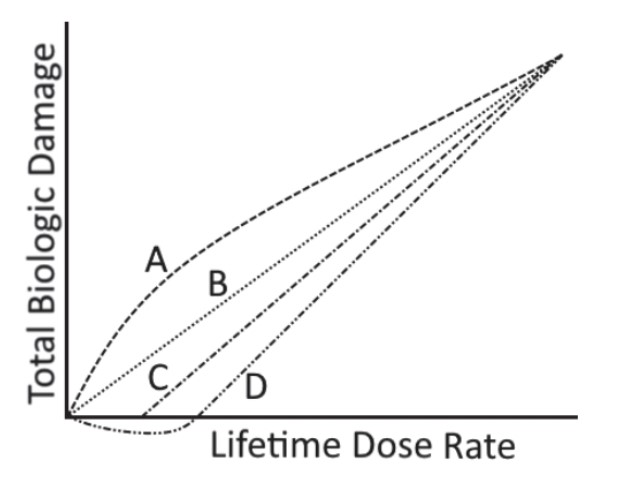
\includegraphics[width=0.5\textwidth]{Imagens/modelosLineares.jpg}
        \end{center}
        
        \item A definição de D\textsubscript{x\%} é “a dose indo para o x\% mais quente do volume”. Da mesma forma, se o volume tivesse sido descrito em termos de número absoluto de cc, em vez de um volume relativo, o D\textsubscript{xcc} denotaria “a dose indo para os x cc mais quentes do volume”. D\textsubscript{xGy} é uma notação imprópria, pois o subscrito deve se referir a um volume, não a uma dose. V\textsubscript{x\%} refere-se ao “volume recebendo x\% da dose”, então V\textsubscript{5\%}= 60 Gy é uma notação imprópria, pois V\textsubscript{x\%} deve relatar um volume, não uma dose. Da mesma forma, V\textsubscript{xcc} é uma notação imprópria, pois o subscrito deve ser um valor de dose relativo ou absoluto, não um valor de volume absoluto.
        
        \item Se a restrição do órgão em risco (OAR) for baseada na dose máxima, não há problema em limitar a segmentação apenas à parte do OAR dentro dos campos de tratamento, pois a dose máxima não pode ser encontrada fora da área irradiada. As restrições D\textsubscript{x\%} , V\textsubscript{x\%} ou V\textsubscript{xGy} podem ou não estar OK, dependendo se o volume absoluto do OAR está incluído nos campos de tratamento. A dose média e as restrições de D\textsubscript{x\%} são baseadas em todo o volume do OAR, portanto sub-segmentar o OAR sempre dará a resposta incorreta.
        
        \item O ITV contabiliza todas as posições que o GTV pode ocupar devido ao movimento respiratório durante o tratamento. Gating respiratório força o feixe a ser ativado apenas durante a parte escolhida do ciclo respiratório; portanto, o feixe não estará ligado quando o GTV estiver em algumas posições (aquelas acima da linha horizontal superior no diagrama). Para obter mais informações sobre gating, consulte o relatório AAPM No. 91, The Management of Respiratory Motion in Radiation Oncology. 
        
        \item Se o único parâmetro DVH de interesse for a dose máxima pontual, basta limitar a segmentação da estrutura à porção da estrutura na área tratada. No entanto, para relatórios precisos de outros parâmetros DVH, toda a estrutura deve ser segmentada. O DVH poderá ser impreciso caso.
        
        \item A expansão de GTV para PTV é um conceito espacial. O GTV é expandido para propagação microscópica para o CTV, que é expandido para movimento interno para o ITV, que é expandido para movimento inter e intrafracional do paciente para o PTV. As incertezas do cálculo da dose não são consideradas no projeto das margens do PTV.
        
        \item de acordo com o formalismo  AAPM TG-263 a dose  solicitada para 95\% do volume alvo em relação à dose prescrita é V5\%\[\%\]A dose em um volume relativo (não absoluto) é especificada em “V5\%” com a dose solicitada “[\%]” relativa à prescrição e em unidades não absolutas.
        
        \item Seguindo a ICRU 62, o PTV é uma expansão do CTV e, portanto, deve incluir todos os voxels dentro do CTV. Se a dose mínima de CTV for menor que a dose mínima de PTV, o PTV não deve estar incluindo esses voxels de dose mínima de CTV, indicando que os volumes foram definidos incorretamente.
        
    \end{itemize}
\end{exemplo}

\bibliography{ref.bib}
\end{document}